\documentclass{article}

% Packages
\usepackage[utf8]{inputenc} % UTF-8 input encoding
\usepackage[T1]{fontenc} % Font encoding
\usepackage{amsmath, amssymb} % Math packages
\usepackage{enumitem} % For customizing lists
\usepackage{lipsum} % For generating dummy text
\usepackage{listings}
\usepackage{graphicx}


\lstset{%
  language=bash,
  basicstyle=\fontfamily{pcr}\selectfont,
  commentstyle=\bfseries,
  escapeinside={(*@}{@*)}
}

\newcommand{\comment}[1]{\# here is a comment: #1}
\newcommand\floor[1]{\lfloor#1\rfloor}
\newcommand\ceil[1]{\lceil#1\rceil}

% Title and author information
\title{Algorithms (6470) HW02}
\author{Alex Darwiche}
\date{\today}

\begin{document}

\maketitle

\section*{Answers}

% Question 1
\subsection*{Q1}
\begin{enumerate}[label=(\alph*)]
    \item Show how partition function would work on Array A<13,19,9,5,12,8,7,4,21,2,6,11>.
    \subitem 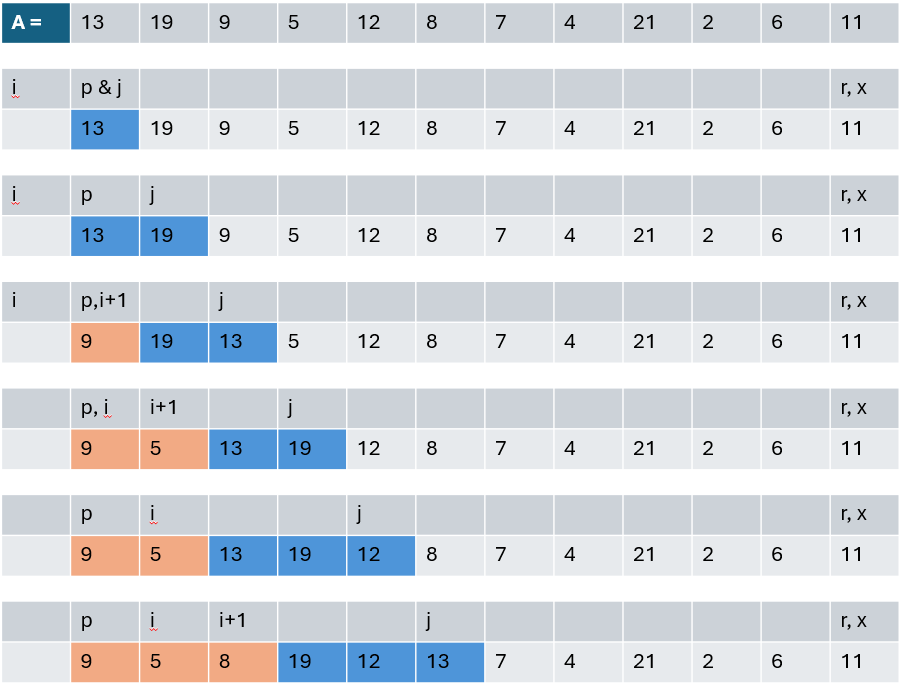
\includegraphics[width=1\textwidth]{partition1.png}
    \subitem 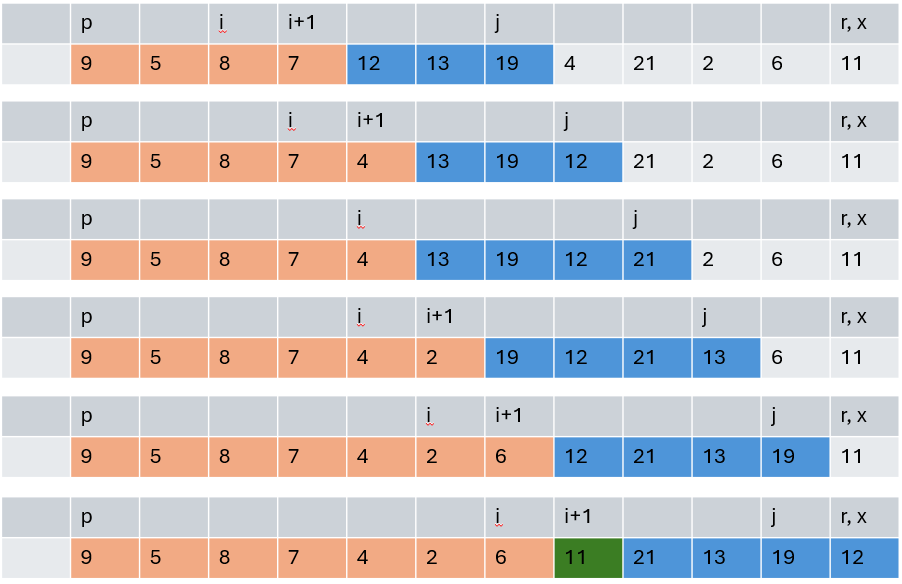
\includegraphics[width=1\textwidth]{partition2.png}
\end{enumerate}

% Question 2
\subsection*{Q2}
\begin{enumerate}[label=(\alph*)]
    \item Show that Quicksort's best case scenario is $\Omega(nlogn)$
    \item First, we need to show that $T(n) \geq cnlogn$
    \item This can be done by finding a $c$ and $n$ where: $T(n) = cnlogn + (something)$
    \item The best case scenario for quicksort is when each of the paritions is equal sized at each step. This would leave a recurrence relationship equivalent to: $T(n) = 2* T(\frac{n}{2}) + \theta(n)$
    \subitem (1) $T(n) \geq cnlogn$
    \subitem (2) $T(\frac{n}{2}) \geq c\frac{n}{2}log\frac{n}{2}$
    \subitem (3) Sub this back into original formula: $T(\frac{n}{2}) = 2*(c\frac{n}{2}log\frac{n}{2}) + \theta(n)$
    \subitem (4) Simplify: $T(\frac{n}{2}) = cn * (logn - log2) + n$
    \subitem (5) Simplify: $T(\frac{n}{2}) = cnlogn - cn + n = cnlogn + n(1-c)$
    \subitem (6) Now we need to solve for where $(1-c) > 0$ or $c < 1$ for all $n>0$

\end{enumerate}

% Question 3
\subsection*{Q3}
\begin{enumerate}[label=(\alph*)]
    \item What do you expect the performance of these algorithms to be on the above dataset?
    \subitem (1) Merge Sort: This sort is $O(nlogn)$ for all cases (Best, Worst, Average). Given this is a partially sorted dataset, this algorithm will do less comparisons than the average case, generally moving closer to the best case scenario. This is because the merge operation can take a short cut when the first partition is all higher/lower than the second partition.
    \subitem (2) Insertion Sort: This sort will do less comparisons than the average case, given the data is partially sorted. Given the data is almost completely sorted, I believe this will be $O(n)$.
    \subitem (3) Heap Sort: This data can quickly be arranged as a heap (there is no build heap needed). This however is still a $O(nlogn)$ and will does the same amount of comparisons as an other array.
    \subitem (4) Quicksort: This sort will likely perform worse than average, given the data is already nearly sorted. Assuming we were to use the first or last element as a pivot, we would be getting heavily unbalanced partitions at each step. This might cause this sort to perform $O(n^2)$. This can be improved likely, with a better pivot selection algorithm if one exists.
    \item Given the data is nearly sorted, I would recommend Insertion Sort for this array. This should operate as $O(n)$.

\end{enumerate}

% Question 4
\subsection*{Q4}
\begin{enumerate}[label=(\alph*)]
    \item Sorted List Decision Tree complexity
    \subitem 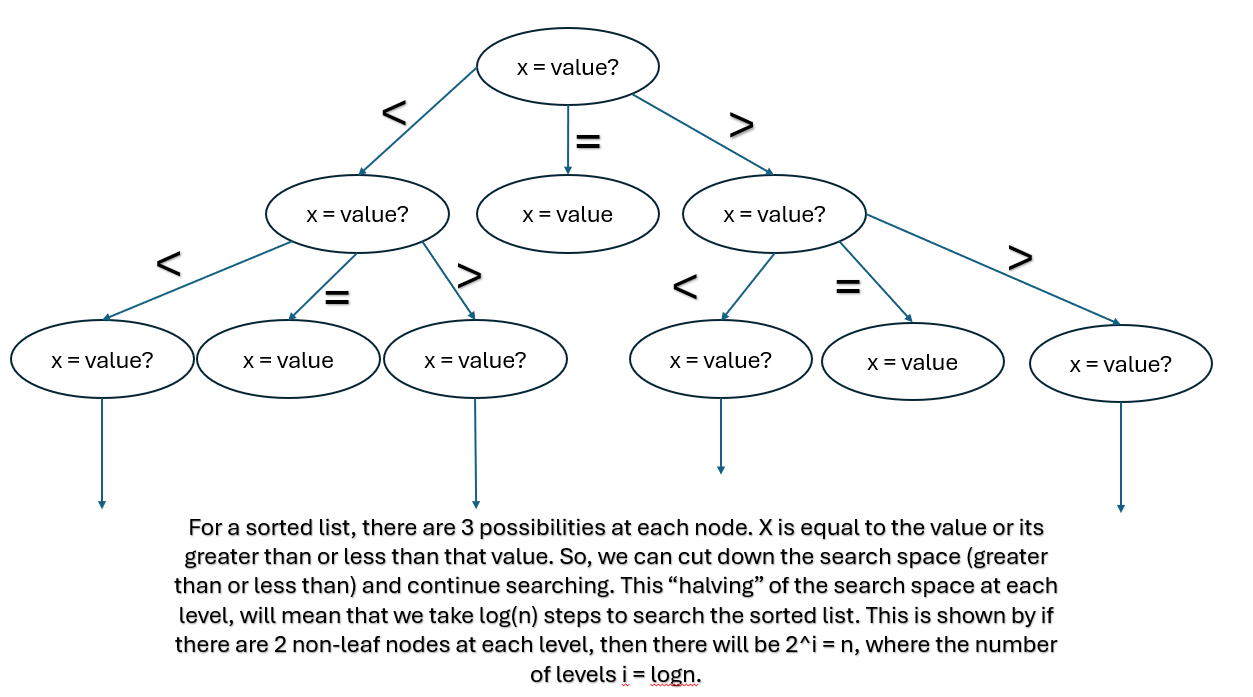
\includegraphics[width=1\textwidth]{sorted.png}

    \item Unsorted List Decision Tree complexity
    \subitem 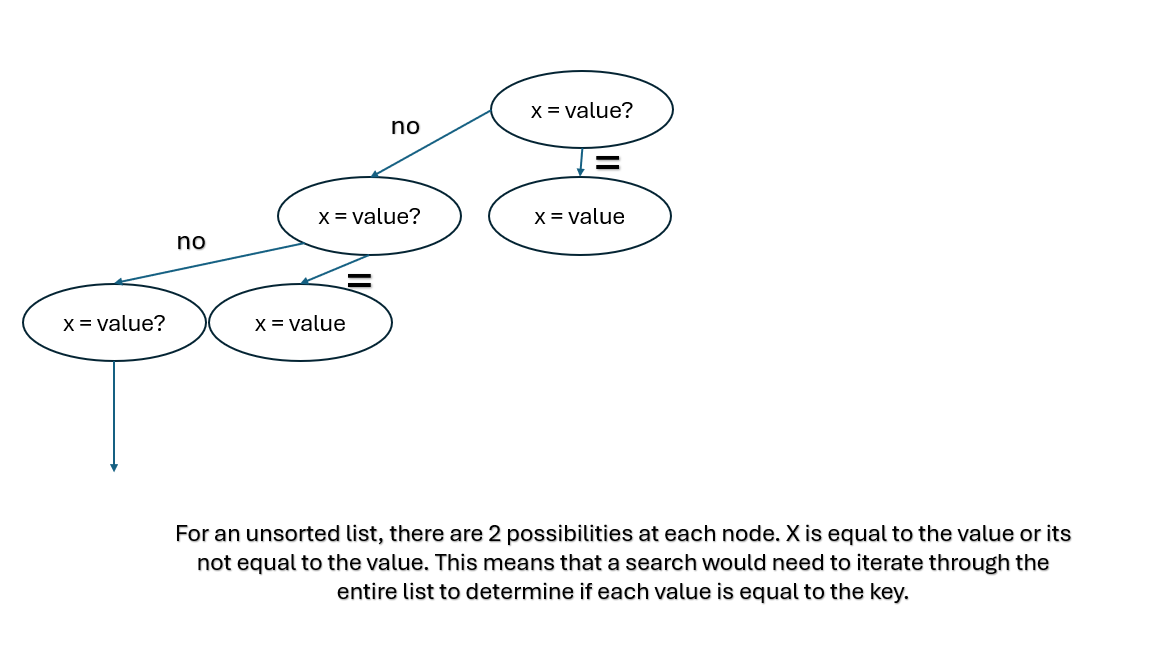
\includegraphics[width=1\textwidth]{unsorted.png}

    \item The lower bound of the complexity is $\Omega(log(n))$ for a sorted list, assuming that each decision point exactly splits the data in half at each step. For an unsorted list, you either need to search each value individually, which is $\Omega(n)$ or you need to sort the list first. Either way, the lower bound is greater than $\Omega(n)$ for an unsorted list. Thus, regardless of if the data is sorted or unsorted, the lower bound complexity will be $\Omega(log(n))$.
\end{enumerate}

% Question 5
\subsection*{Q5}
\begin{enumerate}[label=(\alph*)]
    \item Counting sort on Array A.
    \subitem 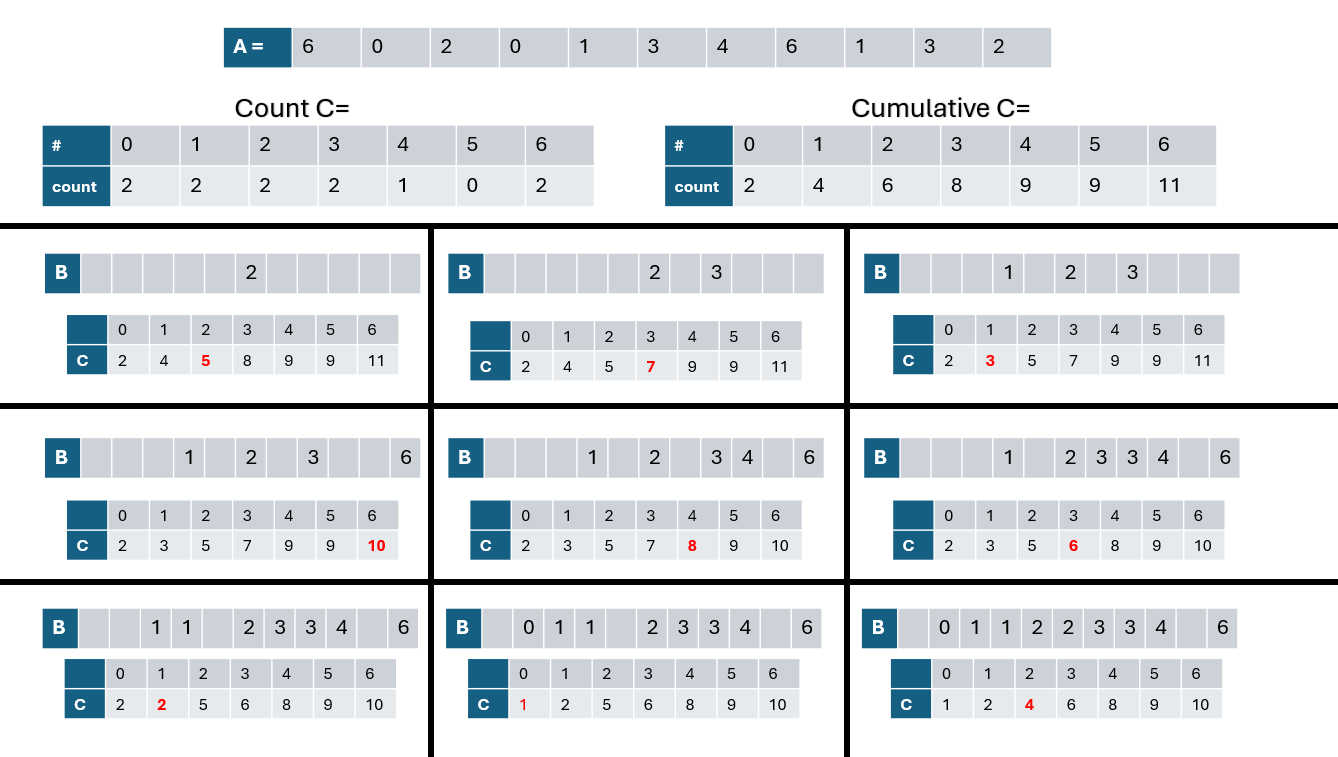
\includegraphics[width=1\textwidth]{counting1.png}
    \subitem 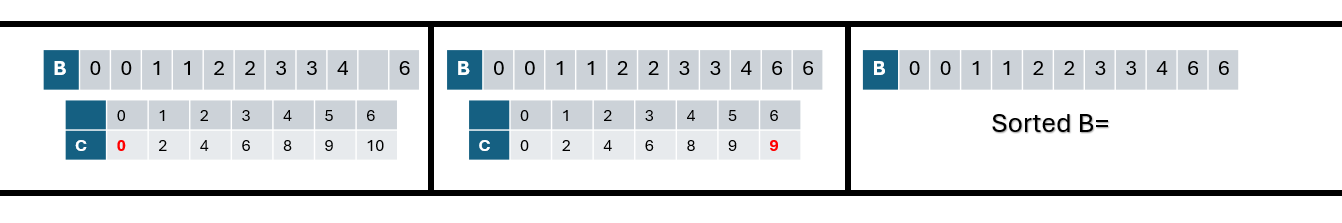
\includegraphics[width=1\textwidth]{counting2.png}
\end{enumerate}

% Question 6
\subsection*{Q6}
\begin{enumerate}[label=(\alph*)]
    \item Radix Sort on 3-letter words array.
    \item \subitem 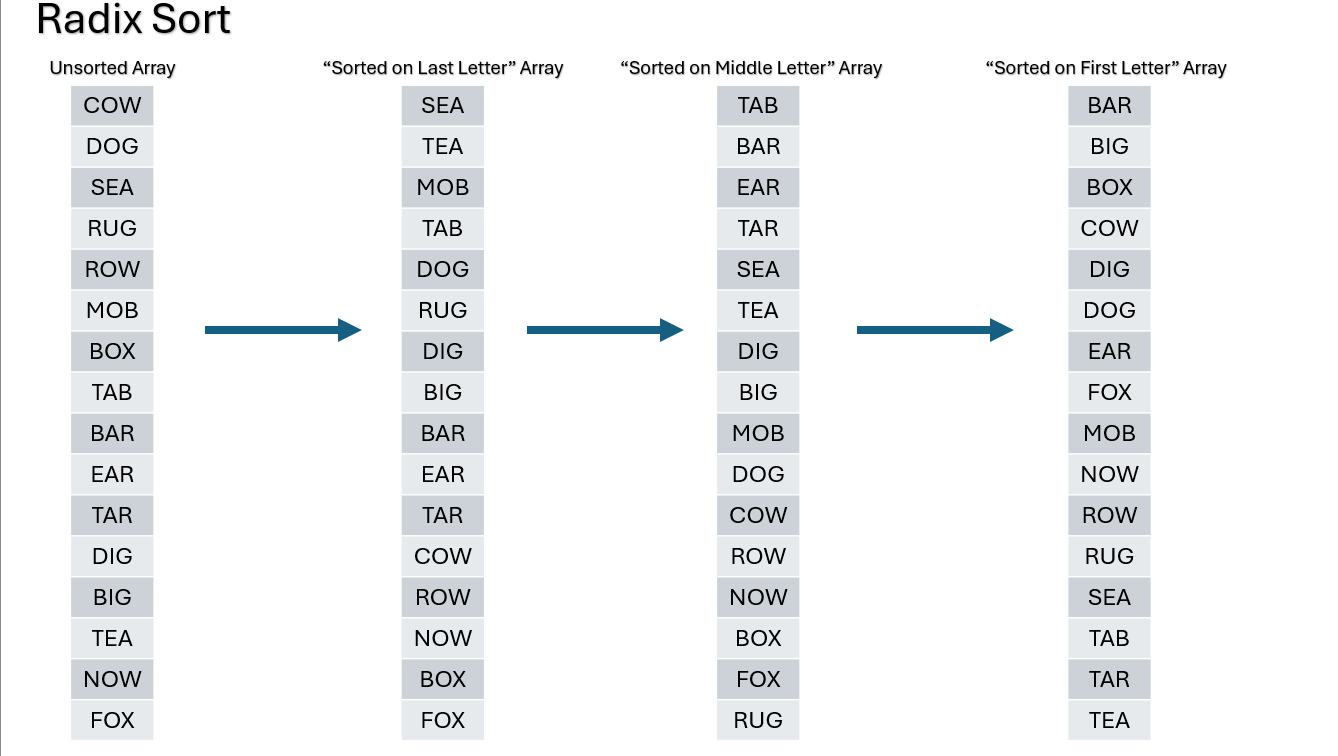
\includegraphics[width=1\textwidth]{radix.png}
\end{enumerate}

% Question 7
\subsection*{Q7}
\begin{enumerate}[label=(\alph*)]
    \item First, prove that groups of 9 would be $O(n)$ in the worst case.
    \subitem (1) Assumptions: $ g \leq \frac{n}{9}$, $9g$ = max total elements, n.
    \subitem (2) Now, to find the worst case scenario, we will find the minimum number of elements less than our median of median x. This should be $\floor{\frac{g}{2}}$ groups, with 5 elements in each group. We need to remove a few elements from this though, to include a partial column and the median itself. So total elements smaller than the median are $5*\floor{\frac{g}{2}} - (4+1)$. 
    \subitem (3) Next, Subtract from total $(9g-4) - [5*(\frac{g}{2}) - 5] \approx \frac{18g}{2} - \frac{5g}{2}$ = $\frac{13g}{2}$
    \subitem (4) We can sub back in $ g \leq \frac{n}{9}$ to get $\frac{13n}{18}$
    \subitem (5) Now, we rewrite our recurrence relationship as: $T(n) = T(\frac{n}{9}) + T(\frac{13n}{18}) + \Theta(n)$
    \subitem (6) To show this is $O(n)$ we need to show that $T(n) \leq cn$
    \subitem (7) $T(\frac{n}{9}) \leq c*\frac{n}{9} $
    \subitem (8) $T(\frac{13n}{18}) \leq  c*\frac{13n}{18}$
    \subitem (9) Subbing back in: $T(n) = c*\frac{n}{9} + c*\frac{13n}{18} + n = c*\frac{15n}{18} + n = cn - c*\frac{3n}{18} + n = cn - n*(\frac{3c}{18}-1)$
    \subitem (10) Lastly, show that $\frac{3c}{18}-1 > 0$, select $c > \frac{18}{3}$ for all n > 0.

    \item Second, show that groups of 3 would not be $O(n)$ in the worst case, repeating all the steps in the first part of this problem.
    \subitem (1) Assumptions: $ g \leq \frac{n}{3}$, $3g$ = max total elements, n.
    \subitem (2) Now, to find the worst case scenario, we will find the minimum number of elements less than our median of median x. This should be $\floor{\frac{g}{2}}$ groups, with 5 elements in each group. We need to remove a few elements from this though, to include a partial column and the median itself. So total elements smaller than the median are $2*\floor{\frac{g}{2}} - (2+1)$. 
    \subitem (3) Next, Subtract from total $(3g-2) - [2*(\frac{g}{2}) - 3] \approx 3g - g$ = $2g$
    \subitem (4) We can sub back in $ g \leq \frac{n}{3}$ to get $\frac{2n}{3}$
    \subitem (5) Now, we rewrite our recurrence relationship as: $T(n) = T(\frac{n}{3}) + T(\frac{2n}{3}) + \Theta(n)$
    \subitem (6) To show this is not $O(n)$ we need to show that $T(n) > cn$.
    \subitem (7) $T(\frac{n}{3}) \leq c*\frac{n}{3} $
    \subitem (8) $T(\frac{2n}{3}) \leq  c*\frac{2n}{3}$
    \subitem (9) Subbing back in: $T(n) = c*\frac{n}{3} + c*\frac{2n}{3} + n = c*n + n$
    \subitem (10) This shows that we will be unable to make this $T(n) \leq cn$, so groups of 3 are not linear.
\end{enumerate}

% Question 8
\subsection*{Q8}
\begin{enumerate}[label=(\alph*)]
    \item Demonstrate the Hoare Partition:
    \subitem 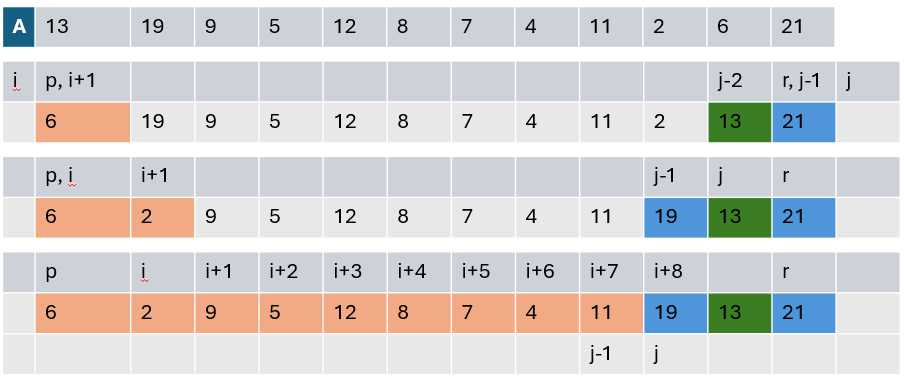
\includegraphics[width=1\textwidth]{hoarePartition.png}

    \item Compare Hoare Partition to normal Partition.
    \subitem (1) The Hoare partition includes the pivot in the arrays that it returns. The return "j" is simply the bound of the lower pivot in Hoare partition, rather than the position of the pivot value in the normal patrition. The Hoare partition works from the front and the back at the same time, whereas the other partition function starts from p and goes till r-1. The Hoare Partition compares each A[i] and A[j] to a value x, rather than comparing two elements of the array together at each step, a subtle difference in their comparisons.

    \item Compare when all the elements are equal.
    \subitem 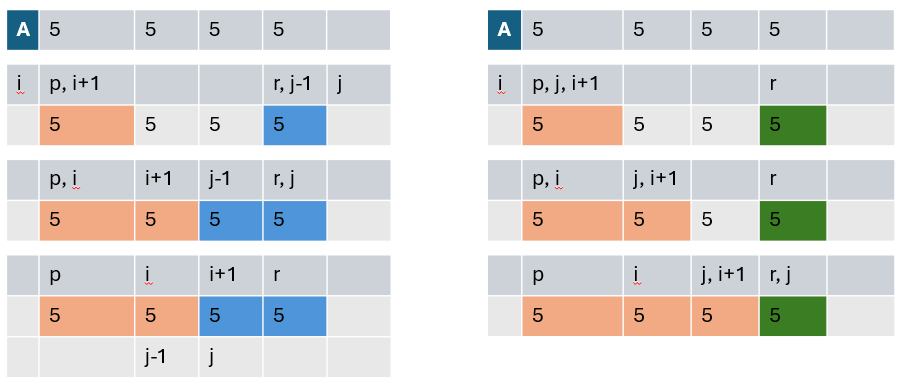
\includegraphics[width=1\textwidth]{comparingPartitions.png}
    \subitem (1) The difference in the total number of steps is equivalent in these two algorithms. The difference in is the returned arrays that get called in the next recurrsive call. Hoare partition appears to return 2 equally (within +1) sized arrays, whereas the normal partition function will return one array that is n-1 length and another that is empty. This will cause the Hoare Partition to perform near best case for quicksort, around $O(nlogn)$ and will cause a Normal Partition quicksort to perform near an $O(n^2)$ complexity.
    \subitem (2) This likely means that a HOARE-PARTITION is good in practice on datasets that have many duplicates.
    
    \item Assuming A[p..r] contains at least two elements, prove i and j never leave A.
    \subitem (1) The Hoare Partition returns when i is greater than or equal to j. So, this means that there are 3 cases can occur in an array.
    \subitem (2) Case 1: The array contains many elements and there are swaps that occur between the indices of i and j. These two indices will eventually crossover one another and terminate at that point, somewhere in the middle of the Array A.
    \subitem (3) Case 2+3: These cases are the edge cases where there are only 2 elements in the array. As you can see in the picture below, the indexing of i and j will cause the recursion to terminate before either i or j exit the bounds of Array A. The red boxes indicate a "terminating" state.
    \subitem 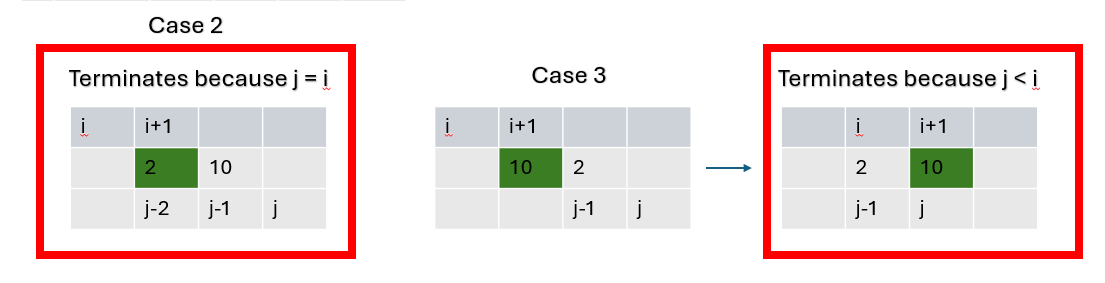
\includegraphics[width=1\textwidth]{cases.png}
    
    \item Prove the return j value is: $p\leq j < r$. 
    \subitem (1) Given i and j never leave the Array A, and that j is incremented down by 1 (at least) each loop. We can say that any Array of size greater than 2, j will be less than r and greater than or equal to p. 
    \subitem (2) The above graphic proves this point for arrays that are size 2, and the same intuition can be extended to larger arrays. j will increment down at least twice in all HOARE-PARTITION'ing. 
    \subitem (3) Perhaps more explicity, in the first iteration, i will always be stopped at the pivot (pivot = A[p]). This means that j will move left until it finds a value that is less than the pivot. If that first value is less than or equal to the pivot, a swap will occur. This then means that that the next iteration, j will decrement at least 1 more, and it will be less than r. If that first value is not less than or equal to the pivot, then j will have been decremented at least twice, again being lower than r. If j is unable to find a value that is less than or equal to the pivot, it will continue until the pivot. This will mean that i and j are equal (in the first iteration) and the Partition will return a j that is equal to p.
\end{enumerate}

% Question 9 (Graduate students only)
\subsection*{Q1 (Graduate students only)}
\begin{enumerate}[label=(\alph*)]
    \item What happens to QUICKSORT if all values are the same.
    \subitem (1) As seen in the above Question #8, we see that the PARTITION function returns 2 partitions, one that is size n-1 and another that is size 0. 
    \subitem (2) This means that the time complexity is $T(n) = T(n-1) + T(0) + \Theta(n)$ = $T(n) = T(n-1) + \Theta(n)$
    \subitem (3) Per the master theorem, we can see this is $O(n^2)$, where a = 1, b = 1, and d=1.
    \subitem (4) To show that $O(nlogn)$ does nto work, we'd use $T(n) \leq cnlogn$ and $T(n-1) \leq c(n-1)log(n-1)$.
    \subitem (5) Subbing back in: $T(n) = c(n-1)log(n-1) + kn$. Given $nlog(n-1) \leq nlogn$, we can sub that in and get $T(n) = cnlog(n) + kn$.
    \subitem (6) As we can see here, there is no way to make $cnlog(n) + kn \leq cnlog(n)$.
    \item How to improve the complexity of the QUICKSORT so it is still $O(nlogn)$.
    \subitem (1) Rather than using the less than or equal to in PARTITION, we could instead create 3 different different brackets where 1. Less Than Pivot, 2. Equal to Pivot, and 3. Greater than Pivot. This will allow the PARTITION function to pass back "complete" when it finds that the size of partitions 1 and 3 are both empty in part a. In my data structures course, we learned quicksort with this approach, essentially grouping all duplicates of the pivot in the middle of the array. 
\end{enumerate}

% Question 10 (Graduate students only)
\subsection*{Q2 (Graduate students only)}
\begin{enumerate}[label=(\alph*)]
    \item Placeholder
    \begin{lstlisting}[frame=single]
        def RANDOMIZED-SELECT-ITERATIVE(A, p, r, i):
        FLAG = TRUE

        while (FLAG == TRUE)
            if p == r:
                return A[p]
            q = RANDOMIZED-PARTITION(A, p, r)
            k = q - p + 1
            if i == k:
                FLAG = FALSE
                value = A[q]
            else if i < k:
                p = p
                r = q-1
                i = i 
            else:
                p = q+1
                r = r
                i = i-k
        return value

        \end{lstlisting}
\end{enumerate}

\end{document}
